\documentclass[12pt,twoside]{article}

\newcommand{\reporttitle}{495 Advanced Statistical Machine Learning and Pattern Recognition}
\newcommand{\reportauthor}{Thomas Teh}
\newcommand{\reporttype}{Coursework 1: Expectation Maximization and Gaussian Mixture Models}
\newcommand{\cid}{0124 3008}

% include files that load packages and define macros
%%%%%%%%%%%%%%%%%%%%%%%%%%%%%%%%%%%%%%%%%
% University Assignment Title Page 
% LaTeX Template
% Version 1.0 (27/12/12)
%
% This template has been downloaded from:
% http://www.LaTeXTemplates.com
%
% Original author:
% WikiBooks (http://en.wikibooks.org/wiki/LaTeX/Title_Creation)
%
% License:
% CC BY-NC-SA 3.0 (http://creativecommons.org/licenses/by-nc-sa/3.0/)
% 
% Instructions for using this template:
% This title page is capable of being compiled as is. This is not useful for 
% including it in another document. To do this, you have two options: 
%
% 1) Copy/paste everything between \begin{document} and \end{document} 
% starting at \begin{titlepage} and paste this into another LaTeX file where you 
% want your title page.
% OR
% 2) Remove everything outside the \begin{titlepage} and \end{titlepage} and 
% move this file to the same directory as the LaTeX file you wish to add it to. 
% Then add \input{./title_page_1.tex} to your LaTeX file where you want your
% title page.
%
%----------------------------------------------------------------------------------------
%	PACKAGES AND OTHER DOCUMENT CONFIGURATIONS
%----------------------------------------------------------------------------------------
\usepackage{ifxetex}
\usepackage{textpos}
\usepackage{natbib}
%\usepackage{breqn}
\usepackage{kpfonts}
\usepackage[a4paper,hmargin=2.8cm,vmargin=2.0cm,includeheadfoot]{geometry}
\usepackage{ifxetex}
\usepackage{stackengine}
\usepackage{tabularx,longtable,multirow,subfigure,caption}%hangcaption
\usepackage{fncylab} %formatting of labels
\usepackage{fancyhdr}
\usepackage{color}
\usepackage[tight,ugly]{units}
\usepackage{url}
\usepackage{float}
\usepackage[english]{babel}
\usepackage{amsmath}
\usepackage{graphicx}
\usepackage[colorinlistoftodos]{todonotes}
\usepackage{dsfont}
\usepackage{epstopdf} % automatically replace .eps with .pdf in graphics
\usepackage{natbib}
\usepackage{backref}
\usepackage{array}
\usepackage{latexsym}
\usepackage{etoolbox}

\usepackage{enumerate} % for numbering with [a)] format 



\ifxetex
\usepackage{fontspec}
\setmainfont[Scale=.8]{OpenDyslexic-Regular}
\else
\usepackage[pdftex,pagebackref,hypertexnames=false,colorlinks]{hyperref} % provide links in pdf
\hypersetup{pdftitle={},
  pdfsubject={}, 
  pdfauthor={\reportauthor},
  pdfkeywords={}, 
  pdfstartview=FitH,
  pdfpagemode={UseOutlines},% None, FullScreen, UseOutlines
  bookmarksnumbered=true, bookmarksopen=true, colorlinks,
    citecolor=black,%
    filecolor=black,%
    linkcolor=black,%
    urlcolor=black}
\usepackage[all]{hypcap}
\fi

\usepackage{tcolorbox}

% various theorems
\usepackage{ntheorem}
\theoremstyle{break}
\newtheorem{lemma}{Lemma}
\newtheorem{theorem}{Theorem}
\newtheorem{remark}{Remark}
\newtheorem{definition}{Definition}
\newtheorem{proof}{Proof}

% example-environment
\newenvironment{example}[1][]
{ 
\vspace{4mm}
\noindent\makebox[\linewidth]{\rule{\hsize}{1.5pt}}
\textbf{Example #1}\\
}
{ 
\noindent\newline\makebox[\linewidth]{\rule{\hsize}{1.0pt}}
}



%\renewcommand{\rmdefault}{pplx} % Palatino
% \renewcommand{\rmdefault}{put} % Utopia

\ifxetex
\else
\renewcommand*{\rmdefault}{bch} % Charter
\renewcommand*{\ttdefault}{cmtt} % Computer Modern Typewriter
%\renewcommand*{\rmdefault}{phv} % Helvetica
%\renewcommand*{\rmdefault}{iwona} % Avant Garde
\fi

\setlength{\parindent}{0em}  % indentation of paragraph

\setlength{\headheight}{14.5pt}
\pagestyle{fancy}
\fancyfoot[ER,OL]{\thepage}%Page no. in the left on
                                %odd pages and on right on even pages
\fancyfoot[OC,EC]{\sffamily }
\renewcommand{\headrulewidth}{0.1pt}
\renewcommand{\footrulewidth}{0.1pt}
\captionsetup{margin=10pt,font=small,labelfont=bf}


%--- chapter heading

\def\@makechapterhead#1{%
  \vspace*{10\p@}%
  {\parindent \z@ \raggedright %\sffamily
        %{\Large \MakeUppercase{\@chapapp} \space \thechapter}
        %\\
        %\hrulefill
        %\par\nobreak
        %\vskip 10\p@
    \interlinepenalty\@M
    \Huge \bfseries 
    \thechapter \space\space #1\par\nobreak
    \vskip 30\p@
  }}

%---chapter heading for \chapter*  
\def\@makeschapterhead#1{%
  \vspace*{10\p@}%
  {\parindent \z@ \raggedright
    \sffamily
    \interlinepenalty\@M
    \Huge \bfseries  
    #1\par\nobreak
    \vskip 30\p@
  }}
  



% %%%%%%%%%%%%% boxit
\def\Beginboxit
   {\par
    \vbox\bgroup
	   \hrule
	   \hbox\bgroup
		  \vrule \kern1.2pt %
		  \vbox\bgroup\kern1.2pt
   }

\def\Endboxit{%
			      \kern1.2pt
		       \egroup
		  \kern1.2pt\vrule
		\egroup
	   \hrule
	 \egroup
   }	

\newenvironment{boxit}{\Beginboxit}{\Endboxit}
\newenvironment{boxit*}{\Beginboxit\hbox to\hsize{}}{\Endboxit}



\allowdisplaybreaks

\makeatletter
\newcounter{elimination@steps}
\newcolumntype{R}[1]{>{\raggedleft\arraybackslash$}p{#1}<{$}}
\def\elimination@num@rights{}
\def\elimination@num@variables{}
\def\elimination@col@width{}
\newenvironment{elimination}[4][0]
{
    \setcounter{elimination@steps}{0}
    \def\elimination@num@rights{#1}
    \def\elimination@num@variables{#2}
    \def\elimination@col@width{#3}
    \renewcommand{\arraystretch}{#4}
    \start@align\@ne\st@rredtrue\m@ne
}
{
    \endalign
    \ignorespacesafterend
}
\newcommand{\eliminationstep}[2]
{
    \ifnum\value{elimination@steps}>0\leadsto\quad\fi
    \left[
        \ifnum\elimination@num@rights>0
            \begin{array}
            {@{}*{\elimination@num@variables}{R{\elimination@col@width}}
            |@{}*{\elimination@num@rights}{R{\elimination@col@width}}}
        \else
            \begin{array}
            {@{}*{\elimination@num@variables}{R{\elimination@col@width}}}
        \fi
            #1
        \end{array}
    \right]
    & 
    \begin{array}{l}
        #2
    \end{array}
    &%                                    moved second & here
    \addtocounter{elimination@steps}{1}
}
\makeatother

%% Fast macro for column vectors
\makeatletter  
\def\colvec#1{\expandafter\colvec@i#1,,,,,,,,,\@nil}
\def\colvec@i#1,#2,#3,#4,#5,#6,#7,#8,#9\@nil{% 
  \ifx$#2$ \begin{bmatrix}#1\end{bmatrix} \else
    \ifx$#3$ \begin{bmatrix}#1\\#2\end{bmatrix} \else
      \ifx$#4$ \begin{bmatrix}#1\\#2\\#3\end{bmatrix}\else
        \ifx$#5$ \begin{bmatrix}#1\\#2\\#3\\#4\end{bmatrix}\else
          \ifx$#6$ \begin{bmatrix}#1\\#2\\#3\\#4\\#5\end{bmatrix}\else
            \ifx$#7$ \begin{bmatrix}#1\\#2\\#3\\#4\\#5\\#6\end{bmatrix}\else
              \ifx$#8$ \begin{bmatrix}#1\\#2\\#3\\#4\\#5\\#6\\#7\end{bmatrix}\else
                 \PackageError{Column Vector}{The vector you tried to write is too big, use bmatrix instead}{Try using the bmatrix environment}
              \fi
            \fi
          \fi
        \fi
      \fi
    \fi
  \fi 
}  
\makeatother

\robustify{\colvec}

%%% Local Variables: 
%%% mode: latex
%%% TeX-master: "notes"
%%% End: 
 % various packages needed for maths etc.
% quick way of adding a figure
\newcommand{\fig}[3]{
 \begin{center}
 \scalebox{#3}{\includegraphics[#2]{#1}}
 \end{center}
}

%\newcommand*{\point}[1]{\vec{\mkern0mu#1}}
\newcommand{\ci}[0]{\perp\!\!\!\!\!\perp} % conditional independence
\newcommand{\point}[1]{{#1}} % points 
\renewcommand{\vec}[1]{{\boldsymbol{{#1}}}} % vector
\newcommand{\mat}[1]{{\boldsymbol{{#1}}}} % matrix
\newcommand{\R}[0]{\mathds{R}} % real numbers
\newcommand{\Z}[0]{\mathds{Z}} % integers
\newcommand{\N}[0]{\mathds{N}} % natural numbers
\newcommand{\nat}[0]{\mathds{N}} % natural numbers
\newcommand{\Q}[0]{\mathds{Q}} % rational numbers
\ifxetex
\newcommand{\C}[0]{\mathds{C}} % complex numbers
\else
\newcommand{\C}[0]{\mathds{C}} % complex numbers
\fi
\newcommand{\tr}[0]{\text{tr}} % trace
\renewcommand{\d}[0]{\mathrm{d}} % total derivative
\newcommand{\inv}{^{-1}} % inverse
\newcommand{\id}{\mathrm{id}} % identity mapping
\renewcommand{\dim}{\mathrm{dim}} % dimension
\newcommand{\rank}[0]{\mathrm{rk}} % rank
\newcommand{\determ}[1]{\mathrm{det}(#1)} % determinant
\newcommand{\scp}[2]{\langle #1 , #2 \rangle}
\newcommand{\kernel}[0]{\mathrm{ker}} % kernel/nullspace
\newcommand{\img}[0]{\mathrm{Im}} % image
\newcommand{\idx}[1]{{(#1)}}
\DeclareMathOperator*{\diag}{diag}
\newcommand{\E}{\mathds{E}} % expectation
\newcommand{\var}{\mathds{V}} % variance
\newcommand{\gauss}[2]{\mathcal{N}\big(#1,\,#2\big)} % gaussian distribution N(.,.)
\newcommand{\gaussx}[3]{\mathcal{N}\big(#1\,|\,#2,\,#3\big)} % gaussian distribution N(.|.,.)
\newcommand{\gaussBig}[2]{\mathcal{N}\left(#1,\,#2\right)} % see above, but with brackets that adjust to the height of the arguments
\newcommand{\gaussxBig}[3]{\mathcal{N}\left(#1\,|\,#2,\,#3\right)} % see above, but with brackets that adjust to the height of the arguments
\DeclareMathOperator{\cov}{Cov} % covariance (matrix) 
\ifxetex
\renewcommand{\T}[0]{^\top} % transpose
\else
\newcommand{\T}[0]{^\top}
\fi
% matrix determinant
\newcommand{\matdet}[1]{
\left|
\begin{matrix}
#1
\end{matrix}
\right|
}



%%% various color definitions
\definecolor{darkgreen}{rgb}{0,0.6,0}

\newcommand{\blue}[1]{{\color{blue}#1}}
\newcommand{\red}[1]{{\color{red}#1}}
\newcommand{\green}[1]{{\color{darkgreen}#1}}
\newcommand{\orange}[1]{{\color{orange}#1}}
\newcommand{\magenta}[1]{{\color{magenta}#1}}
\newcommand{\cyan}[1]{{\color{cyan}#1}}


% redefine emph
\renewcommand{\emph}[1]{\blue{\bf{#1}}}

% place a colored box around a character
\gdef\colchar#1#2{%
  \tikz[baseline]{%
  \node[anchor=base,inner sep=2pt,outer sep=0pt,fill = #2!20] {#1};
    }%
}%
 % short-hand notation and macros


%%%%%%%%%%%%%%%%%%%%%%%%%%%%

\begin{document}
% front page
% Last modification: 2016-09-29 (Marc Deisenroth)
\begin{titlepage}

\newcommand{\HRule}{\rule{\linewidth}{0.5mm}} % Defines a new command for the horizontal lines, change thickness here


%----------------------------------------------------------------------------------------
%	LOGO SECTION
%----------------------------------------------------------------------------------------


\includegraphics[width = 4cm]{./figures/imperial}\\[0.5cm] 

\begin{center} % Center remainder of the page

%----------------------------------------------------------------------------------------
%	HEADING SECTIONS
%----------------------------------------------------------------------------------------
\textsc{\LARGE \reporttype}\\[1.5cm] 
\textsc{\Large Imperial College London}\\[0.5cm] 
\textsc{\large Department of Computing}\\[0.5cm] 
%----------------------------------------------------------------------------------------
%	TITLE SECTION
%----------------------------------------------------------------------------------------

\HRule \\[0.4cm]
{ \huge \bfseries \reporttitle}\\ % Title of your document
\HRule \\[1.5cm]
\end{center}
%----------------------------------------------------------------------------------------
%	AUTHOR SECTION
%----------------------------------------------------------------------------------------

%\begin{minipage}{0.4\hsize}
\begin{flushleft} \large
\textit{Author:}\\
\reportauthor~(CID: \cid) % Your name
\end{flushleft}
\vspace{2cm}
\makeatletter
Date: \@date 

\vfill % Fill the rest of the page with whitespace



\makeatother


\end{titlepage}




%%%%%%%%%%%%%%%%%%%%%%%%%%%% Main document
\section{Exercise I: Implementation of GMMs}
\subsection{Part a}
A Gaussian distribution has an isotropic covariance means its covariance is proportional to the unit covariance, $\lambda \vec{I}$. This implies the covariance will be spherical in the variable space, which in our case (which is a 2-dimensional data), the data points should cluster and form a circle. Given that we can infer that there are 4 Gaussians, we can group the data points into 4 different clusters in yellow and red as in Figure \ref{fig:Covariance} via visual inspection:

\begin{itemize}
	\item \textbf{Yellow areas}: For theses clusters, we can see that the data points are roughly uniformly spread around the center of the yellow regions, forming a circle. Hence, it is reasonable to infer that these 		data points have Gaussian distributions with isotropic covariance.
	\item \textbf{Red areas}: For these cluster, the data points are do not spread uniformly around a center. Instead, the data points have more variance in one of the dimensions. Hence, for these two clusters, we 		can infer that they have Gaussian distributions with anisotropic covariance.	
\end{itemize}

\begin{figure}[H]
	\begin{center}
		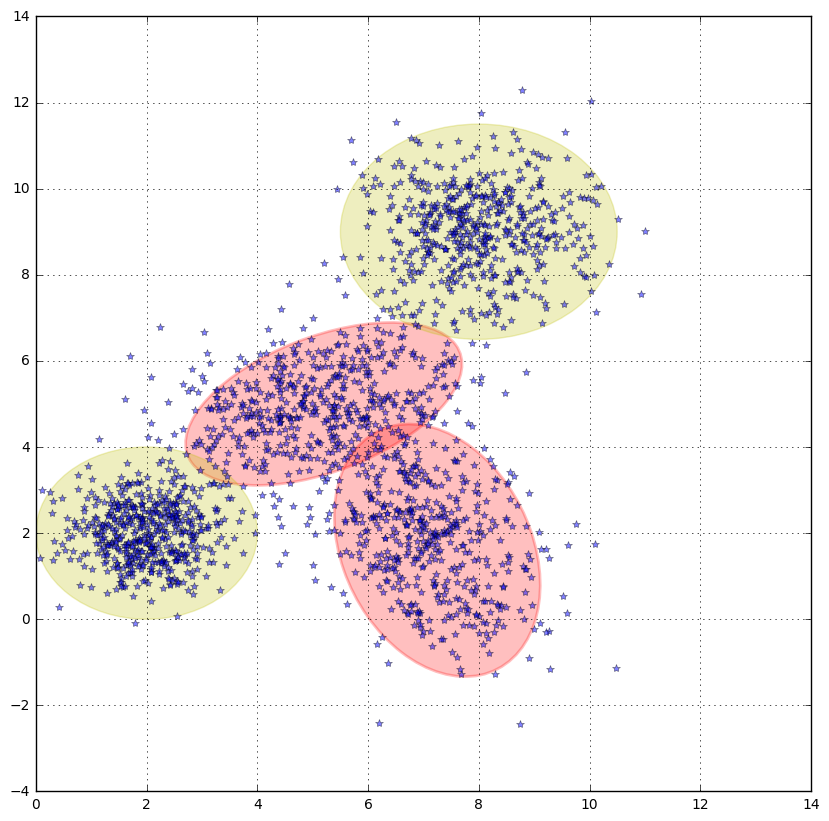
\includegraphics[width = 0.65\hsize]{./figures/CovarianceStructure.png} % this includes the figure and specifies that it should span 0.7 times the horizontal size of the 
		\caption{Covariance structure of the dataset: The yellow areas are circular while the red areas are ellipses. The colored areas are determined merely by eyeballing the data without actually imposing any model 		on it.} % caption of the figure
		\label{fig:Covariance} % a label. When we refer to this label from the text, the figure number is included automatically
	\end{center}
\end{figure}

\subsection{Part b}

\begin{enumerate}
\item \textbf{Random Initialization}: The original function \texttt{random\_params\_generator(K)} in the Python notebook cannot be applied for several reasons.
	\begin{itemize}
		\item The function cannot generate random covariance matrices. Covariance matrices needs to be symmetric and positive semi-definite. By generating a random array of shape (D,D) from the uniform random number generator in Numpy will not work when we input it into the multivariate normal pdf function.
		\item Even if we manage to impose the structure for the covariance matrices, we have an issue of scale. We see that the variables ranges from $-2$ to $14$, which the random number generator generates from a uniform distribution $(0,1)$. In order to use this function, we would need to whiten our data set.
		\item The mixture coefficients are not normalized. Ideally, the sum of the mixture coefficients must be 1. However, this issue does not severely affect the optimization process.
	\end{itemize}

\item \textbf{Random Sampling For Initialization}: I wrote the function \texttt{EMInitRandom(Data, nbCluster, subsampling)} in order to do random initialization.
	\begin{itemize}
		\item Instead of generating random numbers for the parameter values, we do random sampling and estimate the parameters using the random sample from the data set. For each mixture component, we will 	do the random sampling and estimation.
		\item Effectively, we can solve the shortcomings of the previous functions: (1) we can work with data that are not whiten as scale will not be an issue, (2) By default, the estimation will have all the properties of a covariance matrix.
	\end{itemize}

\item \textbf{K-means vs Random Initialization}: When we used the 2nd  method above to initialize the parameters, we find that the algorithm converges much slower relative to k-means initialization. The reason is that the K-means algorithm has already determined the centroids of the clusters. What the GMM does differently from the K-means is merely assigning the data point the probability to which Gaussian distribution it may belong to. In short, K-means algorithm is a hard classification whereas the GMM is a soft classification.

\begin{figure}[H]
	\begin{center}
		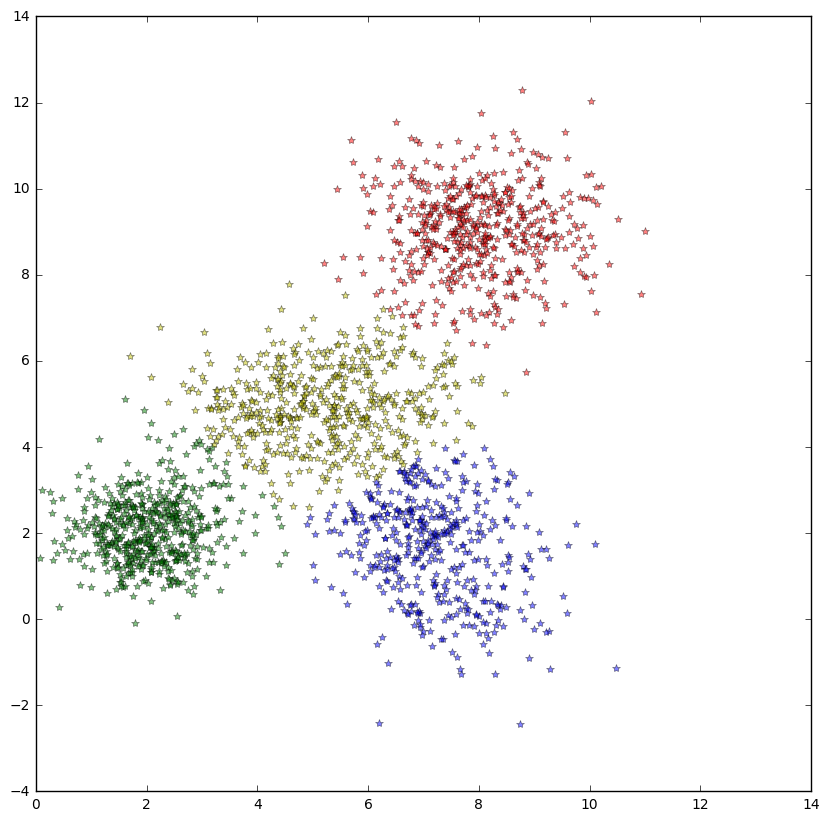
\includegraphics[width = 0.65\hsize]{./figures/KMeans.png} % this includes the figure and specifies that it should span 0.7 times the horizontal size of the 
		\caption{Clustering using K-Means algorithm.} % caption of the figure
		\label{fig:Covariance} % a label. When we refer to this label from the text, the figure number is included automatically
	\end{center}
\end{figure}

\item \textbf{Comment}: From the GMM, we find that indeed that two of the Gaussians have covariances which are close to isotropic while the other two Gaussians' covariances are anisotropic. Please refer to the results from a run of step 10 using the K-means initialization on the next page.


\begin{align*}
\vec{\mu_1}	&= \begin{bmatrix}
7.9763470		&	9.0751523
\end{bmatrix}
\\
\vec{\mu_2}	&= \begin{bmatrix}
7.0258555		&  1.9268015
\end{bmatrix}
\\
\vec{\mu_3}	&= \begin{bmatrix}
5.0051005		&  5.0372016
\end{bmatrix}
\\
\vec{\mu_4}	&= \begin{bmatrix}
1.98810413		&  2.0064038
\end{bmatrix}
\end{align*}

\begin{align*}
\vec{\Sigma_1}&=\begin{bmatrix}
1.0339488		&		 -0.0077491\\
-0.0077491		&  	0.9729311
\end{bmatrix}
\\
\vec{\Sigma_2}&=\begin{bmatrix}
1.0787892		&		-0.5235914\\
-0.5235914  	&		1.9189258
\end{bmatrix}
\\
\vec{\Sigma_3}&=\begin{bmatrix}
1.8969002		&		0.5102359\\
0.5102359		&		0.9838895 
\end{bmatrix}
\\
\vec{\Sigma_4}&=\begin{bmatrix}
0.4927645		& 		0.0065982\\
0.0065982 		&  	0.4585648
\end{bmatrix}
\end{align*}
\begin{align*}
\pi_1 &=0.249784	
\\
\pi_2 &=0.248498
\\
\pi_3 &= 0.250999
\\
\pi_4&=0.250720
\end{align*}

\end{enumerate}

\newpage

\section{Exercise II}
\subsection{Formulation}
Let $\vec{z}$ be a $K$-dimensional binary random variable with 1-of-$K$ representation.
\begin{align*}
p(z_k=1) = \pi_k 	&\Rightarrow p(\vec{z})=\prod_{i=1}^K \pi_k^{z_k}
\end{align*}

Conditional probability of $\vec{x}$ given a particular value for latent variable $\vec{z}$:
\begin{align*}
p(\vec{x}\vert \vec{z}) = \prod_{k=1}^K \mathcal{N}(\vec{x}\vert \vec{\mu}_k, \vec{\Sigma})^{z_k}
\end{align*}

Using Bayes theorem and marginalize the latent variable $\vec{z}$
\begin{align*}
p(\vec{x}) =\sum_{\vec{z}}p(\vec{z})p(\vec{x}\vert \vec{z}) = \sum_{k=1}^K \pi_k\mathcal{N}(\vec{x}\vert \vec{\mu}_k, \vec{\Sigma})
\end{align*}

Similarly, the posterior probability of $\vec{z}$ is given by
\begin{align*}
\gamma (z_k) = \frac{p(\vec{x}\vert \vec{z})p(\vec{z})}{p(\vec{x})} = \frac{\pi_k \mathcal{N}(\vec{x}\vert \vec{\mu}_k, \vec{\Sigma}) }{\sum_{j=1}^K \pi_j\mathcal{N}(\vec{x}\vert \vec{\mu}_j, \vec{\Sigma})}
\end{align*}

\subsection{Expectation Maximization}
\begin{enumerate}
\item Writing down the log-likelihood for the joint distribution:
\begin{align*}
p(\vec{X}, \vec{Z}\vert \vec{\mu}, \vec{\Sigma}, \vec{\pi})& =\prod_{n=1}^{N}\prod_{k=1}^{K} \pi_k^{z_{nk}}\mathcal{N}(\vec{x}_n\vert \vec{\mu}_k, \vec{\Sigma})^{z_{nk}}\\
\ln p(\vec{X}, \vec{Z}\vert \vec{\mu}, \vec{\Sigma}, \vec{\pi})& =\sum_{n=1}^{N}\sum_{k=1}^{K} z_{nk}\left(\ln \pi_k + \ln \mathcal{N}(\vec{x}_n\vert \vec{\mu}_k, \vec{\Sigma})\right)
\end{align*}

\item Taking the expectation on the log likelihood (the E-step):
\begin{align*}
G(\vec{\theta})
& =\mathbb{E}_{p(\vec{Z}\vert \vec{X}, \vec{\theta})}\left[\ln p(\vec{X}, \vec{Z}\vert \vec{\mu}, \vec{\Sigma}, \vec{\pi})\right]\\
& =\sum_{n=1}^{N}\sum_{k=1}^{K} \mathbb{E}_{p(\vec{Z}\vert \vec{X}, \vec{\theta})}[z_{nk}]\left(\ln \pi_k + \ln \mathcal{N}(\vec{x}_n\vert \vec{\mu}_k, \vec{\Sigma})\right)\\
& =\sum_{n=1}^{N}\sum_{k=1}^{K} \gamma(z_{nk})\left(\ln \pi_k -\frac{F}{2}\ln 2\pi -\frac{1}{2}\ln\vert \vec{\Sigma} \vert - \frac{1}{2}(\vec{x_n}-\vec{\mu_k})^\top\vec{\Sigma}^{-1}(\vec{x_n}-\vec{\mu_k})\right)\\
\end{align*}

\item Solving the following optimization problem
\begin{align*}
\max_\vec{\theta} &\text{  } G(\vec{\theta}) -\lambda\left(\sum_{k=1}^K \pi_k -1\right)\\
\textit{s.t.} & \sum_{k=1}^K \pi_k =1
\end{align*}

Let
\begin{align*}
L(\vec{\theta}) & = G(\vec{\theta})-\lambda\left(\sum_{k=1}^K \pi_k -1\right)
\end{align*}

\begin{enumerate}
\item Solving for $\vec{\mu_k}$. We take the derivative of $L(\vec{\theta})$ against $\vec{\mu_k}$
\begin{align*}
\frac{\partial L(\vec{\theta})}{\partial \vec{\mu_k}}
= -\frac{1}{2} \sum_{n=1}^N 2\gamma(z_{nk})\vec{\Sigma^{-1}}(\vec{x_n}-\vec{\mu_k})
= 0\\
\sum_{n=1}^N \gamma(z_{nk})\vec{\Sigma^{-1}}(\vec{x_n}-\vec{\mu_k})=0\\
\sum_{n=1}^N \gamma(z_{nk})\vec{x_n}=\vec{\mu_k}\sum_{n=1}^N \gamma(z_{nk})
\end{align*}

Rearranging the terms
\begin{align*}
\vec{\mu_k} &= \frac{\sum_{n=1}^N \gamma(z_{nk})\vec{x_n}}{\sum_{n=1}^N \gamma(z_{nk})}
\end{align*}

\item Solving for $\vec{\Sigma}$. We take the derivative of $L(\vec{\theta})$ against $\vec{\Sigma}$
\begin{align*}
\frac{\partial L(\vec{\theta})}{\partial \vec{\Sigma}}
=\sum_{n=1}^N\sum_{k=1}^K \gamma(z_{nk})\left(-\frac{1}{2}\vec{\Sigma^{-1}}+\frac{1}{2}\vec{\Sigma^{-1}}(\vec{x_n}-\vec{\mu}_k)(\vec{x_n}-\vec{\mu}_k)^\top\vec{\Sigma^{-1}}\right)=0\\
\sum_{n=1}^N\sum_{k=1}^K \gamma(z_{nk})\left(\vec{1}-(\vec{x_n}-\vec{\mu}_k)(\vec{x_n}-\vec{\mu}_k)^\top\vec{\Sigma^{-1}}\right)=0
\end{align*}

\begin{align*}
\sum_{n=1}^N\sum_{k=1}^K \gamma(z_{nk})\vec{1}=\sum_{n=1}^N\sum_{k=1}^K \gamma(z_{nk})(\vec{x_n}-\vec{\mu}_k)(\vec{x_n}-\vec{\mu}_k)^\top\vec{\Sigma^{-1}}\\
\vec{\Sigma}=\frac{1}{N}\sum_{n=1}^N\sum_{k=1}^K \gamma(z_{nk})(\vec{x_n}-\vec{\mu}_k)(\vec{x_n}-\vec{\mu}_k)^\top
\end{align*}

\item Solving for $\pi_k$. We take the derivative  of $L(\vec{\theta})$ against $\pi_k$ and use the fact that $\sum_{k=1}^K\pi_k=1$
\begin{align*}
\frac{\partial L(\vec{\theta})}{\partial \pi_k}
&= \sum_{n=1}^N\frac{\gamma(z_{nk})}{\pi_k}-\lambda =0\\
\pi_k &=\frac{1}{\lambda}\sum_{n=1}^N\gamma(z_{nk})\\
\sum_{k}^K \pi_k &=\frac{1}{\lambda}\sum_{n=1}^N\sum_{k}^K\gamma(z_{nk})\\
\lambda & = N\\
\pi_k &=\frac{1}{N}\sum_{n=1}^N\gamma(z_{nk})
\end{align*}


\end{enumerate}

\end{enumerate}
\end{document}
%%% Local Variables: 
%%% mode: latex
%%% TeX-master: t
%%% End: 
